\documentclass{article}
\usepackage{geometry}
\geometry{
    a4paper,
    left=30mm,
    right=30mm,
    top=30mm,
    bottom=30mm
}

\usepackage{annotate-equations}
\usepackage{graphicx}
\usepackage{wrapfig}
% \usepackage{figure}

\graphicspath{ {./media/} }
\usepackage[square,numbers]{natbib}
\usepackage[nottoc]{tocbibind}
\usepackage{booktabs}
\usepackage{multirow}
\usepackage{enumitem}
\usepackage{float}

\usepackage{amssymb}
\usepackage{amsmath}

\usepackage{tikz}
\usepackage{listings}
\usepackage{setspace}
\definecolor{Code}{rgb}{0,0,0}
\definecolor{Decorators}{rgb}{0.5,0.5,0.5}
\definecolor{Numbers}{rgb}{0.5,0,0}
\definecolor{MatchingBrackets}{rgb}{0.25,0.5,0.5}
\definecolor{Keywords}{rgb}{0,0,1}
\definecolor{self}{rgb}{0,0,0}
\definecolor{Strings}{rgb}{0,0.63,0}
\definecolor{Comments}{rgb}{0,0.63,1}
\definecolor{Backquotes}{rgb}{0,0,0}
\definecolor{Classname}{rgb}{0,0,0}
\definecolor{FunctionName}{rgb}{0,0,0}
\definecolor{Operators}{rgb}{0,0,0}
\definecolor{Background}{rgb}{0.98,0.98,0.98}
\lstdefinelanguage{Python}{
	numbers=left,
	numberstyle=\footnotesize,
	numbersep=1em,
	xleftmargin=1em,
	framextopmargin=2em,
	framexbottommargin=2em,
	showspaces=false,
	showtabs=false,
	showstringspaces=false,
	frame=l,
	tabsize=4,
	% Basic
	basicstyle=\ttfamily\small\setstretch{1},
	backgroundcolor=\color{Background},
	% Comments
	commentstyle=\color{Comments}\slshape,
	% Strings
	stringstyle=\color{Strings},
	morecomment=[s][\color{Strings}]{"""}{"""},
	morecomment=[s][\color{Strings}]{'''}{'''},
	% keywords
	morekeywords={import,from,class,def,for,while,if,is,in,elif,else,not,and,or,print,break,continue,return,True,False,None,access,as,,del,except,exec,finally,global,import,lambda,pass,print,raise,try,assert},
	keywordstyle={\color{Keywords}\bfseries},
	% additional keywords
	morekeywords={[2]@invariant,pylab,numpy,np,scipy},
	keywordstyle={[2]\color{Decorators}\slshape},
	emph={self},
	emphstyle={\color{self}\slshape},
	%
}

\title{\textbf{Proposal for bachelor thesis}\\
Exploration of the influence of graph parameters on the generalization error of Graph Neural Networks}

\author{Author: Wensheng Zhang}

\date{\today}

\begin{document} 

\maketitle



\begin{abstract}
The goal of this bachelor thesis is to understand empirically how graph parameters/characteristics influence the generalization error of Graph Neural Networks (GNNs).
\end{abstract}


\section{Introduction}\label{sec:intro}

Graph learning became a hot topic in the field of machine learning in recent years. Graph Neural Networks (GNNs), also known as deep learning on graphs, are a class of neural networks that can operate on graph-structured data, such as social networks~\cite{easley2010networks}, biological networks~\cite{barabasi2004network}, and images~\cite{simonovsky2017dynamic}. GNNs use the structure of a graph to perform "message passing", allowing information to propagate across nodes and edges. The key idea is to iteratively aggregate and update node features by exchanging information with local neighboring nodes, which allows GNNs to capture the structural information of the graph. This information is then used to make predictions. GNNs have been demonstrated to be effective in a wide range of tasks, such as node classification~\cite{hamilton2017inductive}, edge prediction~\cite{morselli2021network}, and graph classification~\cite{gilmer2017neural}. Popular GNNs in recent years include Graph Convolutional Networks (GCN)~\cite{kipf2016semi}, Graph Attention Networks (GAT)~\cite{velickovic2020pointer}, and Message Passing Neural Networks (MPNN)~\cite{gilmer2017neural}.  

However, the behavior of GNNs is not well understood. Particularly, the relationship between graph parameters/characteristics and the empirical generalization error of GNNs is not clear.  The goal of this bachelor thesis is to understand empirically how graph parameters/characteristics impact the generalization error of GNNs. 

Before we untangle this problem, we need to define some terms with regard to the graph. In graph theory, we assume that $G=(V,E)$ is an undirected graph, where $V$ is the set of nodes and $E  \subseteq \{\{v,w\}\mid v,w \in V , v \neq w\}$ is the set of edges. We use $\mathbb{G}$ to represent the set of all possible graphs. The neighborhood of a node $v$ is denoted as $N(v)$, defined as $N(v) = \{w \mid \{v,w\} \in E\}$. The degree of a node $v$, denoted as $d(v)$, is the number of neighbors of $v$, that is, $d(v) = |N(v)|$. In addition to the nodes and edges that comprise the graph, we can attach a more complex set of data to each node.  A feature vector $x_n\in \mathbb{R}^k$, is attached to a node $v_n$, and in some cases, edge feature vectors are also included. These vectors can be used to characterize graphs or nodes in graphs. The adjacency matrix $A \in \mathbb{R}^{|V| \times |V|}$ is a matrix that represents the connections between nodes in the graph. The element $a_{ij}$ of the adjacency matrix is 1 if there is an edge between node $v_i$ and node $v_j$, and 0 otherwise.

With these foundational terms in place, we can now introduce the concept of a graph parameter. A graph parameter is a function $f: \mathbb{G} \rightarrow \mathbb{R}^d$ for $d\in \mathbb{N} >0$, which maps a graph to a d-dimensional vector over the reals. Furthermore, such functions need to be permutation invariant, i.e., $f(G) = f(\pi(G))$ for any permutation $\pi$ of the nodes of $G$, where a permutation is a function $\pi: V \rightarrow V$ and $\pi(G)$ denotes the graph obtained by permuting the nodes of $G$ according to $\pi$. A graph parameter allows us to quantify certain properties of a graph, from the basic structural numbers (number of nodes, number of edges, average degree, etc.) to distance properties (average shortest path length, diameter, etc.) to more complex properties (graph clustering coefficient, average number of coloring in the 1-WL algorithm, etc.). This thesis will focus on seven graph parameters, with definitions provided in section~\ref{sec:graph_parameters}.

Additionally, the graph classification task aims to classify a graph into one of several classes. This thesis will specifically focus on addressing this task. A key concept in evaluating model performance or generalization ability in such task is the empirical generalization error $E_{gen}$. This is a measure of how well the model generalizes to unseen data, which can be calculated as the difference between the training accuracy and the test accuracy. It is defined as

$$
    E_{gen} = {Acc_{train}} - {Acc_{test}}
$$
where $Acc_{train}$ is the accuracy of the model on the training dataset, and $Acc_{test}$ is the accuracy of the model on the test dataset. The accuracy $Acc$ on a dataset is defined as the proportion of correctly classified graphs, that is, $Acc = \frac{\text{Number of correctly classified graphs}}{\text{Total number of data points}}$.

The empirical generalization error is also known as the generalization gap~\cite{goodfellow2016deep}. Typically, the learning on the training dataset and test dataset behaves differently. The model may perform well on the training dataset but poorly on the test dataset. By observing the generalization error, we can decide on a stopping criterion for the training process. And the generalization error can be used to determine whether the model is overfitting or underfitting. Furthermore, the generalization error can be influenced by many factors, such as the model architecture, the hyperparameters, and the dataset. In this thesis, I will investigate how the graph parameters influence the generalization error of GNNs. The understanding of the influence of graph parameters on the generalization error of GNNs can help us to understand the behavior of GNNs so that researchers can tune GNNs to improve their predictive performance on new graphs.

\section{Experimental Setup}
The following section outlines the planned methods and materials to be employed in the experiment, including the training framework, the datasets, the models, and the graph parameters.

\subsection{Training Framework}
The training framework is based on PyTorch Geometric~\cite{fey2019fast}. PyTorch Geometric is a library for deep learning on graphs and other irregular structures. It consists of various methods and utilities to ease the implementation of GNNs. 

\subsection{Datasets}
The dataset used for the classification is TUDataset~\cite{morris2020tudataset}. TUDataset is often used for the GNN evaluation. It consists of data from different domains, including small molecules, bioinformatics, social networks and synthetic. Since the size of some datasets is quite small (less than 500 data points/graphs), I will use 10-fold cross validation in the training process, in order to fully utilize the data. A dataset is split into 1:1:8, where one of the folds is treated as the test dataset and another is treated as the validation dataset. The remaining folds are used for training. The training is repeated 10 times, each time with a different test fold. The average of the generalization error over the 10 runs is calculated as the final generalization error of the model. 

\subsection{Models}
In the experiment, I plan to use different GNN layers in the model, including Graph Convolutional Networks(GCN)~\cite{kipf2016semi}, Graph Attention Networks(GAT)~\cite{velickovic2020pointer}, Graph Attention Networks(GATv2)~\cite{brody2021attentive}, Simplified Graph Convolution(SGC)~\cite{wu2019simplifying}, and Message Passing Neural Networks(MPNN)~\cite{gilmer2017neural}. The GCN model is shown in the appendix. The GCN model consists of four GCN layers, each followed by a ReLU activation function. The output of the last GCN layer is passed through a global mean pooling layer, followed by two fully connected layers.

\subsection{Experimental details}
The Adam optimizer~\cite{kingma2014adam} is considered to be employed in the model. To prevent overfitting and to optimize the use of time, the early stopping is employed. The loss function is defined as the cross-entropy loss function. The hyperparameters of the model are considered to be tuned. The hyperparameters include the learning rate, batch size, hidden dimension, number of epochs, and patience in early stopping. The generalization error is calculated as the difference between the training accuracy and the test accuracy.

\subsection{Graph Parameters Under Investigation} \label{sec:graph_parameters}
As graph parameters defined abstractly in the section~\ref{sec:intro}, I give here the concrete definition of the graph parameters.

\begin{description}
    \item [Average degree] The average degree of the graph $d_{avg}$ is defined as the average of the degrees of all nodes in the graph, that is
    $$ d_{avg} = \frac{1}{|V|} \sum_{v \in V} d(v)$$
    \item [Average shortest path length] The average shortest path length of the graph $a$ is defined as the average of the shortest paths between all pairs of nodes in the graph. The shortest path $d(s, t)$ between two nodes $v$ and $w$ is the minimum number of edges that need to be traversed to go from $v$ to $w$. The formal definition is
    $$
a = \frac{1}{|V|(|V|-1)} \sum_{v \in V} \sum_{w \in V, w \neq v} d(v, w)
    $$

    \item [Graph diameter] The graph diameter $d$ is the maximum of the shortest paths between all pairs of nodes in the graph, that is,
    $$
d = \max_{v \in V} \max_{w \in V, w \neq v} d(v, w)
    $$

    \item [Graph density] The graph density $p$ is the ratio of the number of edges in the graph to the number of the maximum possible edges in the graph, that is,
    $$
p = \frac{2|E|}{|V|(|V|-1)}
    $$
    
    \item [Graph clustering coefficient] The graph clustering coefficient $C$ is a measure of the degree to which nodes in a graph tend to cluster together. The clustering coefficient of a node $v$ (as known as the local clustering coefficient) is defined as the fraction of the number of triangles that include node $v$ to the maximum possible number of triples centered on node $v$. The clustering coefficient of the graph (as known as the global clustering coefficient) is defined as the average of the clustering coefficients of all nodes in the graph. The formal definition is
    $$
C = \frac{1}{|V|} \sum_{v \in V} \frac{2\cdot |\{(i,j)\in E \mid i, j \in N(v)\}|}{d(v)(d(v)-1)}
    $$
    where the term $|\{(i,j)\in E \mid i, j \in N(v)\}|$ is the number of edges between the neighbors of node $v$, i.e. the number of triangles containing node $v$. Furthermore, the term $\sum_{v \in V} \frac{2\cdot |\{(i,j)\in E \mid i, j \in N(v)\}|}{d(v)(d(v)-1)}$ is the sum of the local clustering coefficients of all nodes in the graph, in which the degree of node $v$ is denoted as $d(v)$.

    \item [Centrality measure of graphs] At first we have the definition of centrality measure in the \textbf{node level}. The centrality measure of a node is a measure of the importance of the node in the graph. There are many centrality measures, such as degree centrality, closeness centrality, betweenness centrality, and eigenvector centrality. 
    
    \textit{Degree centrality} is identical to the average degree of the graph defined above. 
    
    \textit{Closeness centrality} $C_C(v)$ is defined as the reciprocal of the sum of the length of the shortest paths from the node $v$ to all other nodes in the graph, that is 
    $$C_C(v) = \frac{1}{\sum_{w\in V}{d(v ,w)}}$$
    where $d(v, w)$ is the shortest path between node $v$ and node $w$. 
    
    \textit{Betweenness centrality} $C_B(v)$ is the sum of the fraction of the shortest paths between all pairs of nodes that pass through node $v$, that is
    
    $$
        C_B(v) = \sum_{s,t \in V} \frac{\sigma_{st}(v)}{\sigma_{st}}
    $$
    where $\sigma_{st}$ is the number of the shortest paths between nodes $s$ and $t$, and $\sigma_{st}(v)$ is the number of the shortest paths between nodes $s$ and $t$ that pass through node $v$.
    
    \textit{Eigenvector centrality} is a measure of the influence of a node in a graph based on the concept that connections to high-scoring nodes contribute more to the score of the node in question. Formally, the eigenvector centrality $C_E(v)$ of a node $v$  is defined as the $v$-th component of the eigenvector corresponding to the largest eigenvalue of the adjacency matrix $A$ of the graph. Mathematically, it can be expressed as:
    
    \[ C_E(v) = \frac{1}{\lambda} \sum_{u \in N(v)} a_{vu} C_E(u) \]
    
    where $ \lambda$ is the largest eigenvalue of the adjacency matrix $A$.
$a_{vu}$ is the element of the adjacency matrix $A$ corresponding to the edge between nodes $v$  and $u$.
$ C_E(u)$  is the eigenvector centrality of node $u$.


    Finally, in the \textbf{graph level}, the centrality measure of the graph is defined as the average of the centrality measures over all nodes in the graph.

    \item [Average number of coloring in the 1-WL algorithm] 
    \sloppy
    The 1-dimensional Weisfeiler-Leman algorithm (1-WL)~\cite{weisfeiler1968reduction} is an algorithm that assigns a unique label(color) to each node in the graph, also known as color refinement. The average number of coloring in the 1-WL algorithm is defined as the average number of colors used to color the nodes in the graph. The 1-WL algorithm is a powerful graph isomorphism algorithm that can be used to determine if two graphs are isomorphic. I give the procedure of the 1-WL algorithm here:
    \begin{enumerate}
        \item Assign the same color to all nodes in the graph.
        \item Two nodes $v$, $u$ are assigned a different color if there is a color c such that the number of c-colored neighbors of $u$ is not equal to the number of c-colored neighbors of $v$.
        \item Repeat step 2 until the colors of all nodes do not change.
    \end{enumerate}
    
\end{description}


\section{Results of early experiment} \label{sec:results}

Here I took ten datasets from TUDataset as examples. The calculated parameters are shown in Table~\ref{tab:parameter}. The generalization error of the models are shown in Table~\ref{tab:error}. 


\begin{table}[h!]
    \centering
    \begin{tabular}{@{}lll@{}}
    \toprule
    \multicolumn{1}{c}{\multirow{2}{*}{Dataset}} & \multicolumn{2}{c}{Parameter}                                            \\ \cmidrule(l){2-3} 
    \multicolumn{1}{c}{}                         & \multicolumn{1}{c}{Ave. degree} & \multicolumn{1}{c}{Ave. shortest path} \\ \midrule
    Mutagenicity                                 & 2.0379         & 4.4825                     \\
    NCI1                                         & 2.1550         & 5.4697                     \\
    COIL-RAG                                     & 1.8277         & 1.0606                     \\
    Letter-high                                  & 1.8896         & 1.5173                     \\
    DD                                           & 4.9790         & 7.9700                     \\
    PROTEIN\_full                                & 3.7346         & 4.7123                     \\
    COLORS-3                                     & 2.9288         & 2.0945                     \\ 

    AIDS  &  2.01286  & 3.2864 \\
    ENZYMES  &  3.8626  & 4.4461 \\
    Cuneiform  &  4.0795  & 2.24442 \\ \bottomrule

    \end{tabular}
    \caption{The calculated parameters from a set of datasets, here used two parameters, the average degree of the graph and the average shortest path of the graph which defined in the section \ref{sec:graph_parameters}.}
    \label{tab:parameter}
\end{table}

\begin{table}[h!]
    \centering
    \begin{tabular}{@{}lll@{}}
    \toprule
    Dataset        & Ave. generalization error & Standard Deviation   \\ \midrule
    Mutagenicity   & 0.0268      & 0.02335 \\
    NCI1           & 0.0138      & 0.02649 \\
    COIL-RAG       & 0.0450      & 0.01378 \\
    Letter-high    & 0.0403      & 0.04342 \\
    DD             & 0.0524      & 0.05849 \\
    PROTEINS\_full & 0.0189      & 0.05032 \\
    COLORS-3       & 0.0076      & 0.01428 \\
    AIDS           &  0.00931    & 0.008642 \\
    ENZYMES           &  0.0345    & 0.052339 \\
    Cuneiform           &  0.2392    & 0.09868 \\ \bottomrule
    \end{tabular}
    \caption{The table shows the calculated generalization error from a set of datasets, where the generalization error is calculated as the difference between the training accuracy and the test accuracy.}
    \label{tab:error}
\end{table}

Also, I used a scatter plot to visualize the generalization error against the two graph parameters. The result is shown in Figure~\ref{fig:scatter}. Also, I calculated the correlation between the generalization error and the graph parameters. The result is shown in Table~\ref{tab:correlation}.

\begin{figure}[h!]
    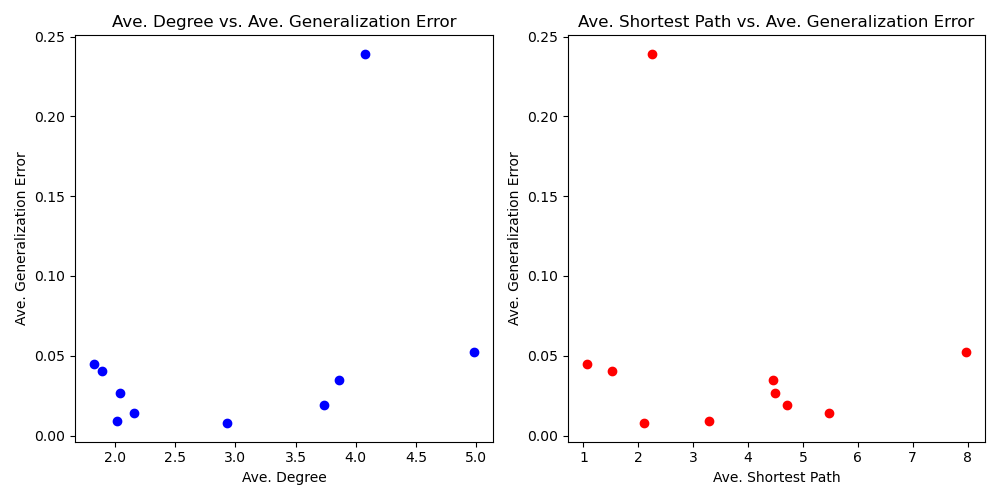
\includegraphics[width=\textwidth]{final_results.png}
    \caption{The generalization error against the graph parameters, the x-axis is the average degree of the graph, the y-axis is the generalization error of the model. Each point in the plot is the calculated result from different datasets (see the table~\ref{tab:parameter}). It is obvious that more datasets are needed to get more reliable results.}
    \label{fig:scatter}
\end{figure}


\begin{table}[ht]
    \centering
    \begin{tabular}{@{}ll@{}}
    \toprule
                       & Ave. Generalization Error \\ \midrule
    Ave degree            & 0.4068                    \\
    Ave. shortest path & -0.2074                   \\ \bottomrule
    \end{tabular}
    \caption{The correlation between the generalization error and the graph parameters. The correlation is calculated by the Pearson correlation coefficient.}
    \label{tab:correlation}
    \end{table}

\newpage

\section{Objective of the thesis}

\begin{figure}[h!]
    \centering
    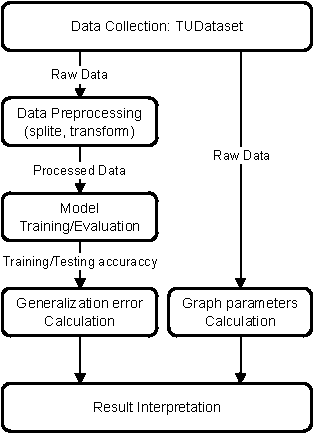
\includegraphics[width=0.5\textwidth]{experiment_procedure.pdf}
    \caption{An illustration of experiment Procedure}
    \label{fig:experiment}
\end{figure}

The Objective of this bachelor thesis is to understand empirically how graph parameters/characteristics influence the generalization error of GNNs. 

In the section~\ref{sec:schedule}, I give the preliminary schedule of the thesis. The thesis will be divided into seven parts: Introduction, Experimental setup, Result, Discussion, Conclusion, References, and Appendix. 

The methodologies of the experiment is described in the figure~\ref{fig:experiment}. The experiment consists of three parts: 1. Train the models from datasets and evaluate the models to calculate the generalization error. 2. Calculate the parameters of the graphs from the dataset. 3. Analyze the influence of the graph parameters on the generalization error of the GNNs.

The following questions will be addressed in the thesis:
\begin{itemize}[noitemsep]
    \item How do different GNN layers perform on different graph parameters? (the methodologies)
    \item How do graph parameters influence the generalization error of GNNs? (the results)
\end{itemize}

The following GNN layers will be explored in the experiment:
\begin{itemize}[noitemsep]
    \item Graph Convolutional Networks(GCN)~\cite{kipf2016semi}
    \item Graph Attention Networks(GAT)~\cite{velickovic2020pointer}
    \item GATv2~\cite{brody2021attentive}
    \item Simplified Graph Convolution(SGC)~\cite{wu2019simplifying}
    \item Message Passing Neural Networks(MPNN)~\cite{gilmer2017neural}
\end{itemize}

The following graph parameters will be explored in the experiment:
\begin{itemize}[noitemsep]
    \item Average degree
    \item Average shortest path length
    \item Graph diameter
    \item Graph density
    \item Graph clustering coefficient
    \item Centrality measure of graphs
    \item Average number of coloring in the 1-WL algorithm
\end{itemize}

Furthermore, it is necessary to adjust the hyperparameters, including the learning rate, batch size, hidden dimension, number of epochs, and patience in early stopping for the models and datasets under consideration.

In the section~\ref{sec:results}, I ran the experiment on 10 datasets. In the future, the experiment will be repeated on a larger number of datasets to enhance the reliability of the results.

\newpage

\section{Preliminary Schedule} \label{sec:schedule}

\begin{itemize}

\item
  1. Introduction
\item
  2. Background on learning on graphs
\item
  2.1 Notation
\item
  2.2 Machine learning
\item
  2.3 Graph neural networks
\item
  2.4 Graph parameters
\item
  3. Experimental study
\item
  3.1 Experimental setup
\item
  3.2. Results
\item
  3.3. Discussion
\item
  6. Conclusion
\item
  7. References
\item
  9. Appendix

\end{itemize}

\clearpage

\bibliographystyle{abbrvnat}
\bibliography{main} % refers to example.bib

\clearpage

\section{Appendix} 
 
\subsection*{Example of GCN model}

\begin{lstlisting}[language=Python]
import torch
from torch import nn
import torch.nn.functional as F
from torch_geometric.nn import GCNConv
from torch_geometric.nn import global_mean_pool


class GCN(torch.nn.Module):
    def __init__(self, in_channels, hidden_channels, out_channels):
        super().__init__()
        self.conv1 = GCNConv(in_channels, hidden_channels)
        self.conv2 = GCNConv(hidden_channels, hidden_channels)
        self.conv3 = GCNConv(hidden_channels, hidden_channels)
        self.conv4 = GCNConv(hidden_channels, hidden_channels)
        self.fc1 = nn.Linear(hidden_channels, hidden_channels)
        self.fc2 = nn.Linear(hidden_channels, out_channels)


    def forward(self, x, edge_index, batch, edge_weight=None):
        x = self.conv1(x, edge_index, edge_weight).relu()
        x = self.conv2(x, edge_index, edge_weight).relu()
        x = self.conv3(x, edge_index, edge_weight).relu()
        x = self.conv4(x, edge_index, edge_weight).relu()
        x = global_mean_pool(x, batch)
        x = self.fc1(x).relu()
        x = self.fc2(x)
        return x
    
    def reset_parameters(self):
        for (_, module) in self._modules.items():
            module.reset_parameters()

\end{lstlisting}

\end{document}